\documentclass[hyperref={pdfpagelabels=false},xcolor=dvipsnames]{beamer}
\usepackage[T1]{fontenc}
\usepackage[utf8x]{inputenc}
\usepackage{amsmath,amsfonts,amssymb}
\usepackage{lmodern}
\usepackage{ngerman}
\usepackage{graphicx}
\usepackage{pdfpages}
\usepackage{remreset}
\usepackage{verbatim} 
\usepackage{listings}
\usepackage{courier}
\lstset{
	basicstyle=\footnotesize\ttfamily,
		showstringspaces=false,
		numbers=left,
		tabsize=4,
		extendedchars=true,
		frame=single,
		frame=topline,
		xleftmargin=20pt,
		framexleftmargin=20pt,
		framextopmargin=3pt,
		framexbottommargin=3pt,
		language=Java
}
\usepackage{caption}
\DeclareCaptionFont{listingcaptions}{\color{black}}
\captionsetup[lstlisting]{
	labelfont=listingcaptions,
		textfont=listingcaptions,
		singlelinecheck=false,
		margin=0pt,
		font={bf,footnotesize}
}

\usetheme{SchulePresentation}
\useinnertheme{circles}

\beamertemplatenavigationsymbolsempty

\title[Bytehawks SE]{Clipboardmanager}
\author[F. Nehrke\and S. Sperling\and T. Schult\and W. Rydzewski]{
	{\sc Felix Nehrke\and Simon Sperling\and Tobias Schult\and Wojciech Rydzewski}}
\institute{Bytehawks SE}
\date{25.05.2012}

\begin{document}

\frame[plain]{
	\titlepage
}

\frame{
	\tableofcontents
}

\section{Einleitung}
\begin{frame}{Einleitung}
	\begin{block}{Was ist der Clipboardmanager?}<+->
		Bearbeitungstool für Clipboardeinträge
	\end{block}
	\begin{block}{User Interface}<+->
		Eine funktionale GUI steht im Vordergrund
	\end{block}
\end{frame}


\section{Profile / Parser}
\begin{frame}{Profile / Parser}
	\begin{block}{Profil}
		Speichern von unterschiedlichen Einstellungen
	\end{block}
	\begin{block}{Parser}
		Veränderung der kopierten Daten
	\end{block}
	\begin{block}{Vorschau}
		Ein Beispiel wie diese Komponenten interagieren
	\end{block}
\end{frame}

\subsection{Parser - unter der Haube}
\begin{frame}[fragile]{Parser - unter der Haube}
\begin{lstlisting}[caption=RegExParser.java]{turnier}
public RegExParser() {
  params = new HashMap<String, Object>();
  params.put("match", "");
  params.put("replace", "");
  name = "RegEx Parser";
}

public String parse(String input) {
  return input.replaceAll(
    (String)params.get("match"), 
    (String)params.get("replace")
  );
}
\end{lstlisting}
\end{frame}


\section{Observer}
\begin{frame}{Observer}
	\begin{block}{Was ist ein Observer?}<+->
		Ein Observer überwacht andere Objekte
	\end{block}
	\begin{block}{Wann ist ein Observer besonders sinnvoll?}<+->
		Um unabhänig vom Rest zu arbeiten
	\end{block}
	\begin{block}{Warum haben wir einen Observer eingesetzt?}<+->
		Wir haben ausgelagerte Threads per Observer eingebunden
	\end{block}
\end{frame}
\subsection{Observer OOD}
\begin{frame}{Observer OOD}
	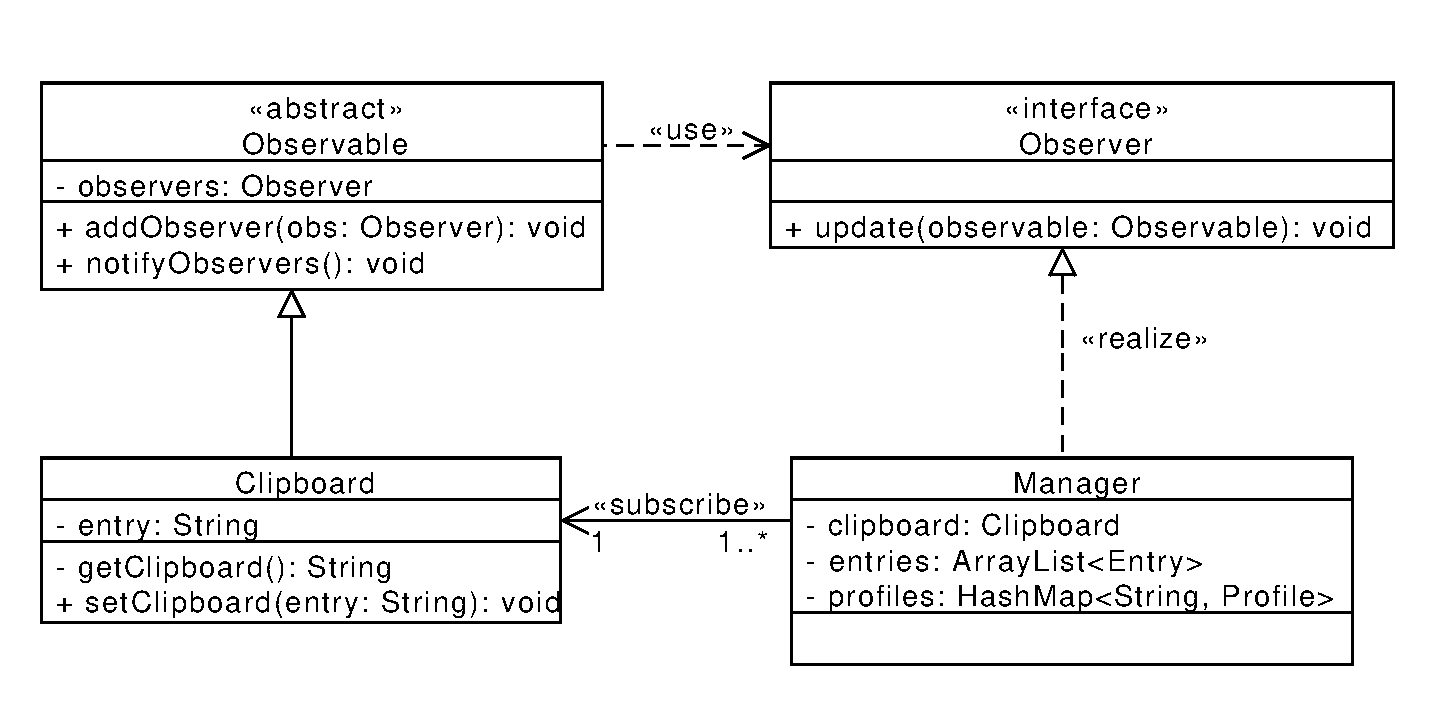
\includegraphics[width=\dimexpr\textwidth]{observerEx.pdf}
\end{frame}


\section{Pluginsystem}
\begin{frame}{Das Plugin-System}
	\begin{columns}
		\column{.453\textwidth}<+->
			\begin{block}{Warum ein Plugin-System?}
				Eine flexible Möglichkeit den Clipboardmanager zu erweitern.
			\end{block}
		\column{.453\textwidth}<+->
			\begin{block}{Wie wurde es umgesetzt?}
				Durch Interfaces werden Standardfunktionen vorgegeben.
			\end{block} 
	\end{columns}
	\begin{block}{Der Pluginloader}<+->
		Es werden alle Jars im Ordner "`plugins"' auf Kompabilität geprüft. Die
		so gefundenen Plugins werden indiziert und gestartet.
	\end{block}
\end{frame}



\section{Abschluss}
\setlength{\parskip}{1em} 
\begin{frame}{Abschluss}
	\begin{block}{Vielen Dank für Ihre ungeteilte Aufmerksamkeit}
		Viel Spaß im Wochende
	\end{block}
	\begin{block}{Website}
		https://github.com/nemoinho/Clipboard-school
	\end{block}
\end{frame}


\end{document}
